\documentclass[border=0.8ex,svgnames,tikz]{standalone}
\usepackage{amsmath,mathtools}
\usepackage{fontspec}
\setmainfont{Source Serif 4}
\setsansfont{Source Sans 3}
\setmonofont{Source Code Pro}
\begin{document}
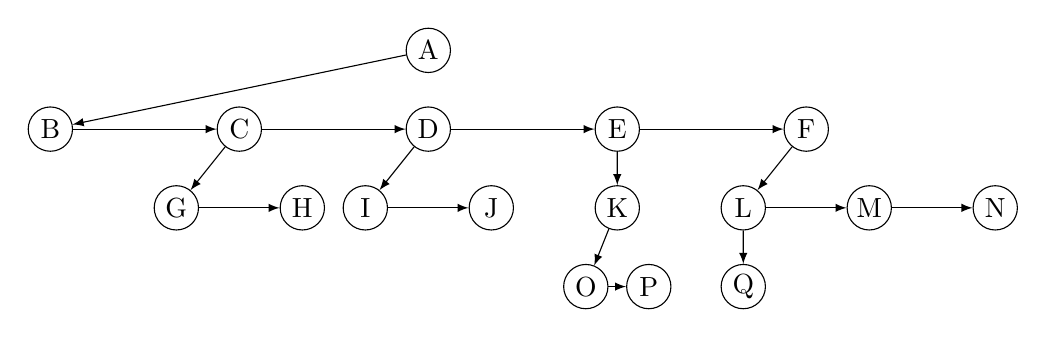
\begin{tikzpicture}[
  level distance=10mm,
  every node/.style={draw,circle,inner sep=1pt,minimum size=1.6em},
  level 1/.style={sibling distance=24mm},
  level 2/.style={sibling distance=16mm},
  level 3/.style={sibling distance=8mm},
  edge from parent/.style={draw=none},
  ]
  \node(a){A}
  child{ node(b){B} }
  child{ node(c){C} child{ node(g){G} } child{ node(h){H} } }
  child{ node(d){D} child{ node(i){I} } child{ node(j){J} } }
  child{
    node(e){E}
    child{ node(k){K} child{ node(o){O} } child{ node(p){P} } }
  }
  child{
    node(f){F}
    child[missing]
    child{ node(l){L} child{ node(q){Q} } }
    child{ node(m){M} }
    child{ node(n){N} }
  };
  \path[draw,>=latex]
  (a) edge[->] (b)
  (b) edge[->] (c)
  (c) edge[->] (g)
  (g) edge[->] (h)
  (c) edge[->] (d)
  (d) edge[->] (i)
  (i) edge[->] (j)
  (d) edge[->] (e)
  (e) edge[->] (k)
  (k) edge[->] (o)
  (o) edge[->] (p)
  (e) edge[->] (f)
  (f) edge[->] (l)
  (l) edge[->] (q)
  (l) edge[->] (m)
  (m) edge[->] (n);
\end{tikzpicture}
\end{document}
